The Volatility GPLVM (V-GPLVM) model is a generalization of the GPLVM model, as discussed in section \ref{sec:models}, where the volatility is reinterpreted as a time dependent quantity. Using the equations and generating process from section \ref{sec:v_gplvm}, we arrive at the model code found in \ref{sec:model_code}. Due to the large number of parameters that need to be stored in RAM at a time, the size of the data matrix $Y$ had to be sufficiently smaller, $Y\in\mathbb{R}^{N,D}=\mathbb{R}^{10,250}$. We find that the model does not apply well to the data, which can be seen from the kernel density estimates of the distributions of noise ($\sigma_n$) and variance ($\Sigma$) values in figures \ref{fig:vola_noises} and \ref{fig:vola_variances}. These estimates should not be having large parts of the estimation reach be outside $\mathbb{R}_0^+$, as this is forbidden by design. In addition, the values should not center around 1, again solidifying the evidence of a corrupted model. Also note, that 
\begin{equation}%eq:variance_volatility
	\Sigma \propto \log(\Sigma_V),
	\label{eq:variance_volatility}
\end{equation}
the variance $\Sigma$ is proportional to the logarithm of the volatility $\log(\Sigma_V)$. The values of the covariance entries, which mainly lie at value $1$ suggest, that the model finds and stays in a steep local minima on the energy surface, which seems unshirkable. It does not seem to be the global minimum though, since covariance entry values, ELBO values and $R^2$ values are far off from where we would expect them to be \ref{fig:vola_ELBO_R2}. We again see that the linear kernel under performs significantly, especially when looking at the volatility values, which need to be way higher, or even unreasonably high for the under performing model. More sophisticated kernels perform better in all tests, and again higher numbers of latent dimensions perform better than lower numbers. If we look at the results, we again can conclude, that not even all model specifications have landed securely in the suspected local minimum due to major differences in ELBO values and $R^2$ values. Also, the $R^2$ values shown in \ref{fig:vola_ELBO_R2} lead to the wrong conclusion, since they only can compare lower dimensional representations of the distributions. 
\begin{figure}[t]%fig:vola_noises
	\centering
	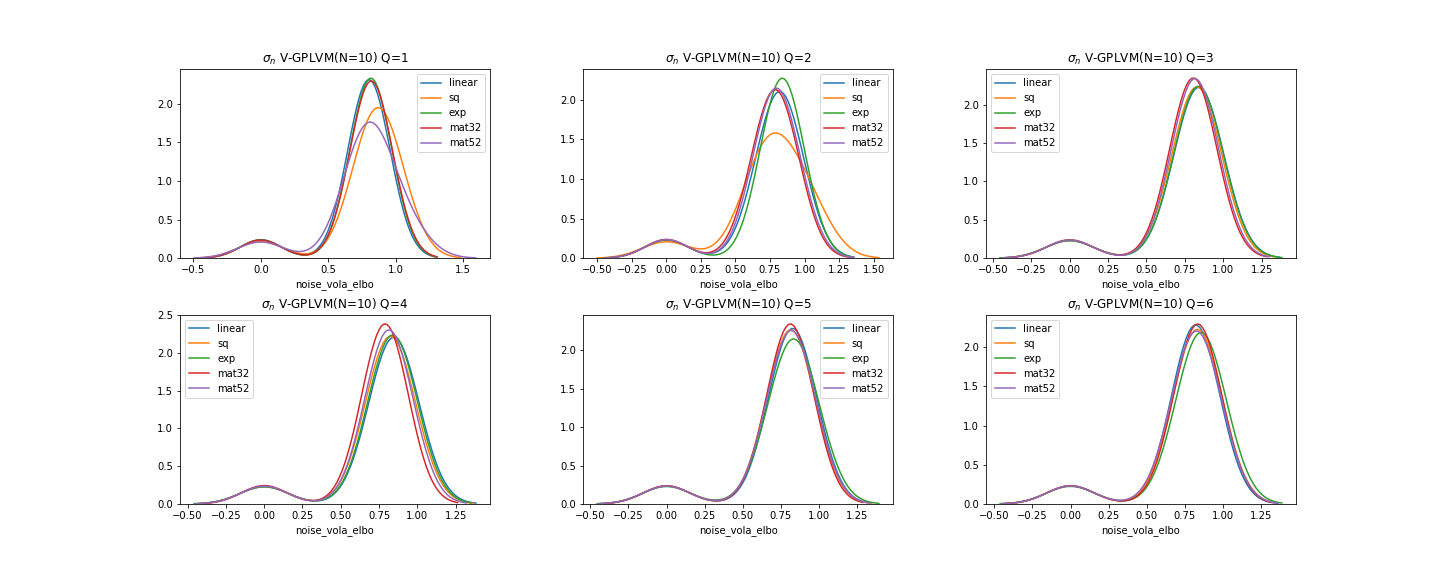
\includegraphics[width=7in]{img/07_2/noise_VOLA_elbo.png}
	\caption[V-GPLVM noise distributions]{V-GPLVM noise distributions for the $N=10$, $D=250$ data set.}
	\label{fig:vola_noises}
\end{figure}
\begin{figure}[b]%fig:vola_variances
	\centering
	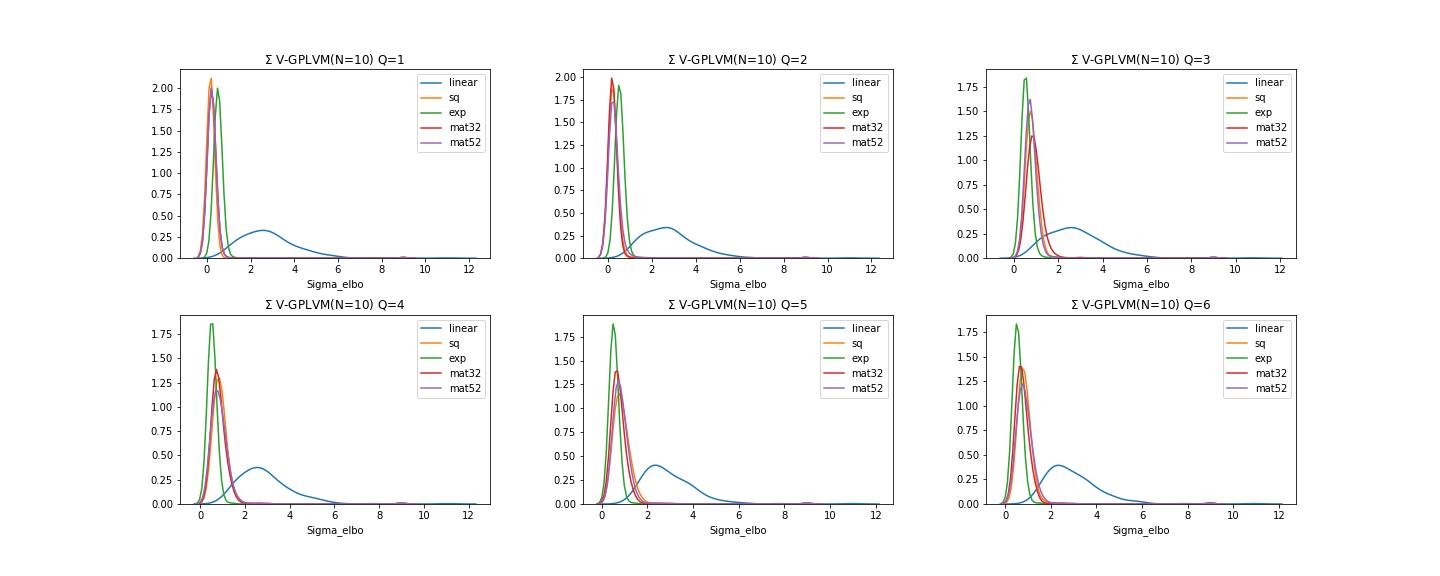
\includegraphics[width=7in]{img/07_2/Sigma_VOLA_elbo.png}
	\caption[V-GPLVM Variance distributions]{V-GPLVM Variance distributions for the $N=10$, $D=250$ data set.}
	\label{fig:vola_variances}
\end{figure}
\begin{figure}[t]
	\centering
	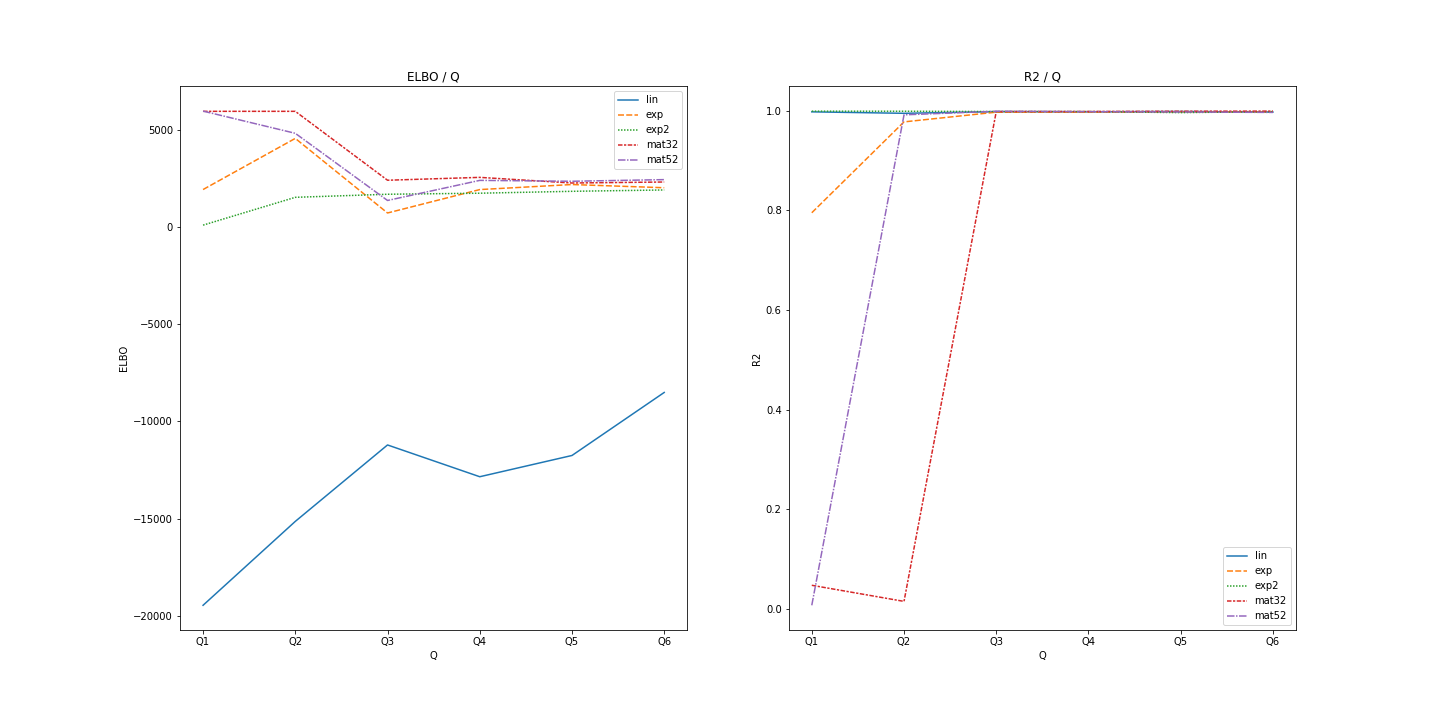
\includegraphics[width=7in]{img/07_2/modelVOLA_Qs.png}
	\caption[V-GPLVM ELBO and $R^2$ model results]{ELBO and R2 values grouped by number of latent dimensions ($Q$) for the V-GPLVM model.}
	\label{fig:vola_ELBO_R2}
\end{figure}
Due to the differences in size in $Y$, these results can not be compared to the GPLVM results directly, but indirectly through looking at the behavior of the model reconstructing the input data in figures \ref{fig:vola_N10_pairs}. These plots again show the same erroneous behavior as the GPLVM model, with a lot of stocks being represented with circle-like shape (\textit{left}) that reproduces the distribution well, but does not reconstruct the higher dimensional representation of the pair plot correctly. This behavior can e.g. inflate $R^2$ values, misleading the reader. The \textit{center} frame shows the erroneous behavior found in the GPLVM model, where to match the distributions, some predictions are falsely set to 0. 
\begin{figure}[b]%fig:vola_N10_pairs
	\centering
	\begin{subfigure}[l]{0.3\textwidth}
		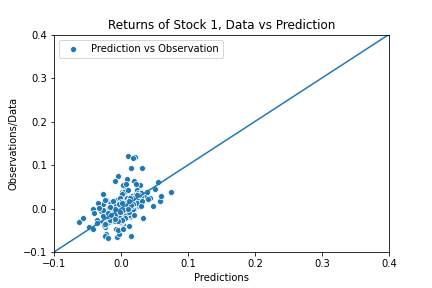
\includegraphics[width=\textwidth]{img/07_2/elbo/Q1_kernel1_stock1_scatter.png}
	\end{subfigure}
	\begin{subfigure}[c]{0.3\textwidth}
		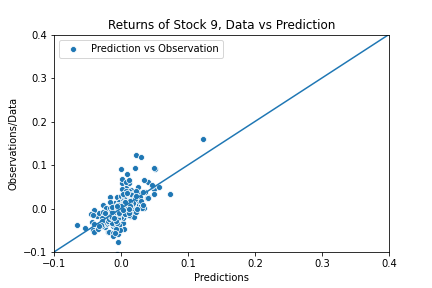
\includegraphics[width=\textwidth]{img/07_2/elbo/Q1_kernel1_stock9_scatter.png}
	\end{subfigure}
	\begin{subfigure}[r]{0.3\textwidth}
		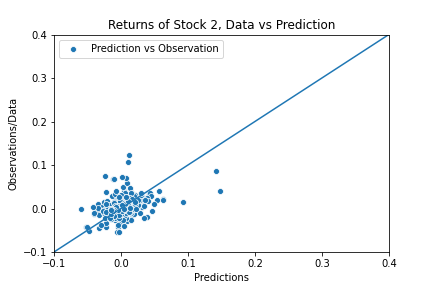
\includegraphics[width=\textwidth]{img/07_2/elbo/Q1_kernel1_stock2_scatter.png}
	\end{subfigure}
	\caption[Y-$\hat{Y}$ pair plots V-GPLVM model]{Y-$\hat{Y}$ pair plots with the V-GPLVM model $N=10$, $D=250$.}
	\label{fig:vola_N10_pairs}
\end{figure}
Also, we can observe the behavior of the model simply underestimating high returns and overestimating low returns, so that the intercept is far off the desired value of 1. This leads directly to the slope, figure \ref{fig:vola_slopes}, and intercept, figure \ref{fig:vola_intercepts}, distributions of the V-GPLVM model. 
\begin{figure}[t]%fig:vola_slopes
	\centering
	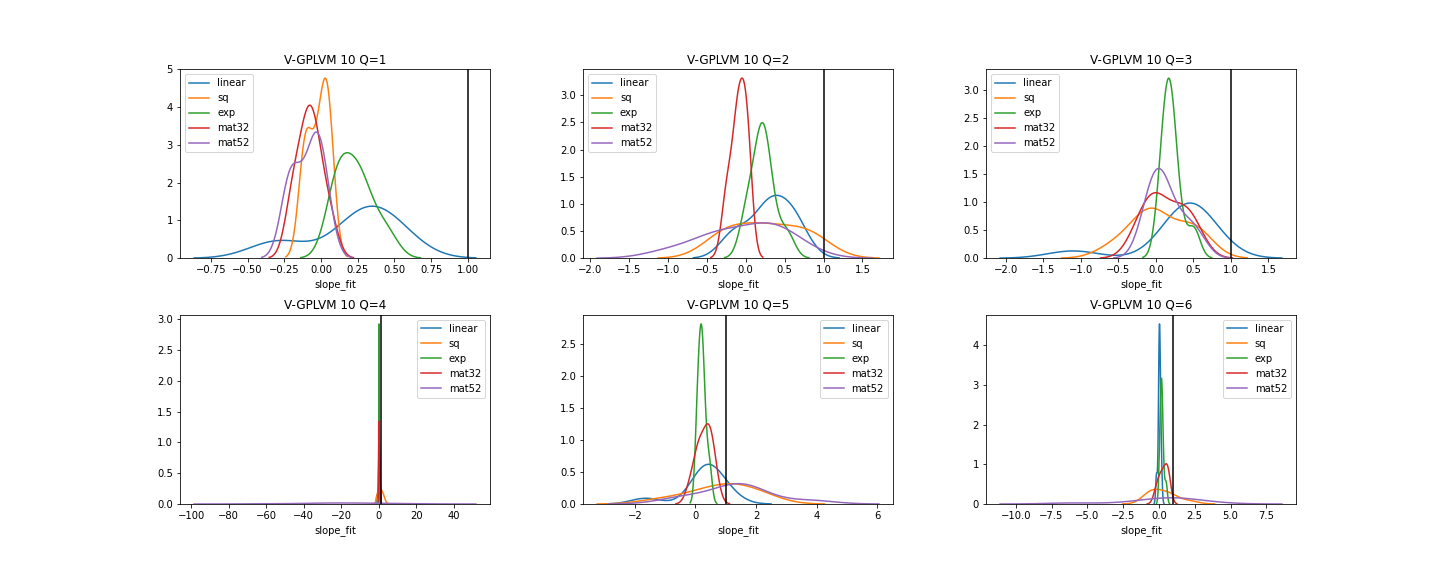
\includegraphics[width=7in]{img/07_2/slope_fit_vola_elbo.png}
	\caption[V-GPLVM slopes distributions]{V-GPLVM slopes distributions for the $N=10$, $D=250$ data set.}
	\label{fig:vola_slopes}
\end{figure}
\begin{figure}[b]%fig:vola_intercepts
	\centering
	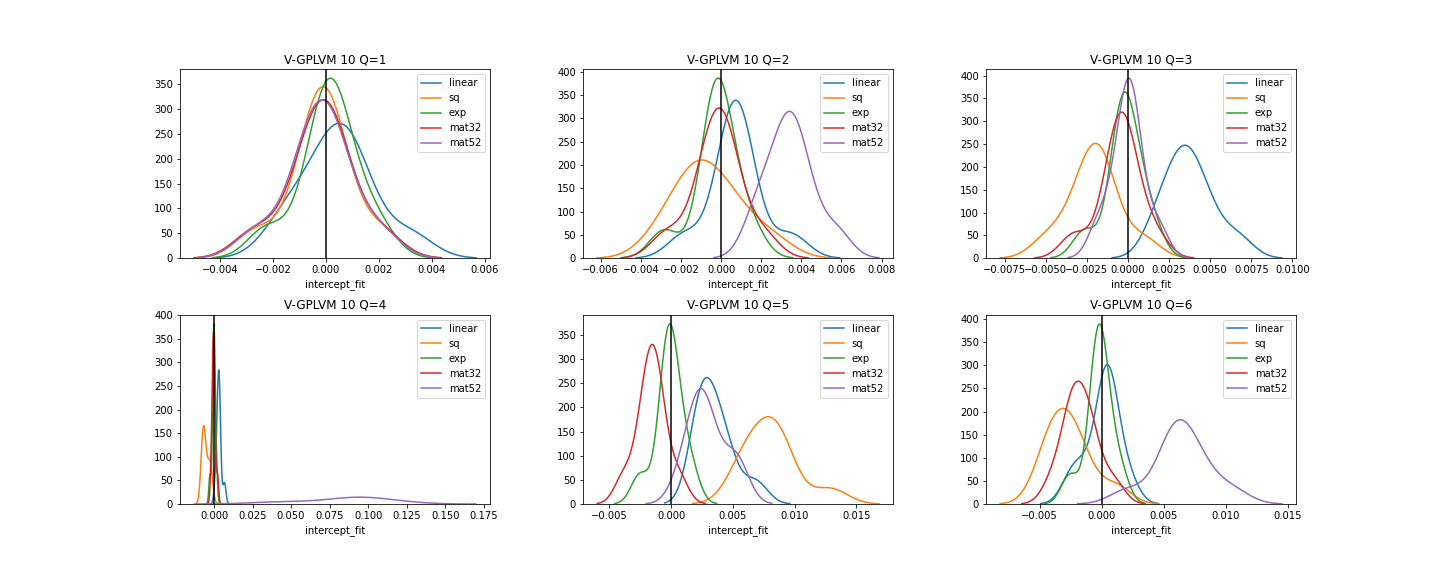
\includegraphics[width=7in]{img/07_2/intercept_fit_vola_elbo.png}
	\caption[V-GPLVM intercepts distributions]{V-GPLVM intercept distributions for the $N=10$, $D=250$ data set.}
	\label{fig:vola_intercepts}
\end{figure}
Again, the model did not initialize sufficiently well with the volatility normalized data sets, as to provide an interpretation. Compared to the other models previously discussed, the slope and intercept distributions giving a quick overview of all the different possible Y-$\hat{Y}$-pair plots, are far off from the optimum. Therefore, we conclude that the model, even though not explicitly comparable, does not measure up with the previous models. 